\chapter{Grundlagen}
Hier erklärt man Grundlagen.

Als Beispiel wird hier schon mal ein Bild eingefügt, damit ein neuer Bachelorand wei\ss{} wie das geht.

\begin{figure}
	\centering
		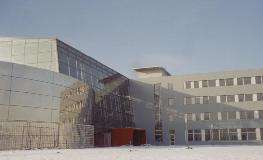
\includegraphics{bilder/garching.jpg}
	\caption{Bild der Mathe und Info Gebäudes in Garching b. München}
	\label{fig:garching}
\end{figure}

Als Beispiel kommen die Worte Grundlagen und Einleitung in den Index \index{Grundlagen} \index{Einleitung}

%%%%%%%%%%%%%%%%%%%%%%%%%%%%%%%%%%%%%%%%%%%%%%%%%%%%%%%%%%%%%%%%%%%%%%%%%%%%%%%
% *** Gleichungen ***
%%%%%%%%%%%%%%%%%%%%%%%%%%%%%%%%%%%%%%%%%%%%%%%%%%%%%%%%%%%%%%%%%%%%%%%%%%%%%%%
%
\section{Gleichungen}\label{sec:gleichungen}
%
Dies ist eine einfache Gleichung
%
\begin{eqnarray}\label{gl:einfache_gleichung}
  y & = & ax^2 + bx + c
\end{eqnarray}



\section{Quellcode}
Man kann mit \LaTeX{} super Quelltext oder Snippets setzen. Dazu muss man die Sprache konfigurieren und wie man möchte, dass der Quellcode aussieht. Das kann pro Snippet passieren. . 
\lstset{
	numbers=left, numberstyle=\tiny, numbersep=5pt,
basicstyle=\small, % print whole listing small 
%keywordstyle=\ttb\color{deepblue}
%identifierstyle=, % nothing happens 
%commentstyle=\color{white}, % white comments 
%stringstyle=\ttfamily, % typewriter type for strings 
%showstringspaces=false} % no special string spaces
}
\begin{lstlisting}[columns=fullflexible,showspaces=false,showtabs=false, language=Python, frame=single, caption={Fakultaetsberechnung}]
def factorial(num): 
  if num < 0: 
      print("Factorial of negative num does not exist")
  elif num == 0: 
    return 1
  else: 
  fact = 1
  while(num > 1): 
    fact *= num 
    num -= 1
  return fact 
\end{lstlisting}

\section{Tabellen}
Tabellen sind ebenfalls gleitende Objekte so wie Bilder. 
\begin{table}
	\centering
	\begin{tabular}{c|c}
		\textbf{Spalte 1} & \textbf{Spalte 2} \\
		\hline
		\hline
		Eintrag & Eintrag \\
		\hline
	\end{tabular}
	\caption{Eine Tabelle}
\end{table}